\documentclass[tikz,border=20pt]{standalone}
\usetikzlibrary{calc,arrows.meta,positioning}
\usepackage{amsmath,amssymb}

\definecolor{clientbg}{HTML}{E0F2FE}
\definecolor{clientborder}{HTML}{0284C7}
\definecolor{gwbg}{HTML}{F3E8FF}
\definecolor{gwborder}{HTML}{9333EA}
\definecolor{idpbg}{HTML}{FEF3C7}
\definecolor{idpborder}{HTML}{D97706}
\definecolor{rsbg}{HTML}{DCFCE7}
\definecolor{rsborder}{HTML}{16A34A}

\begin{document}
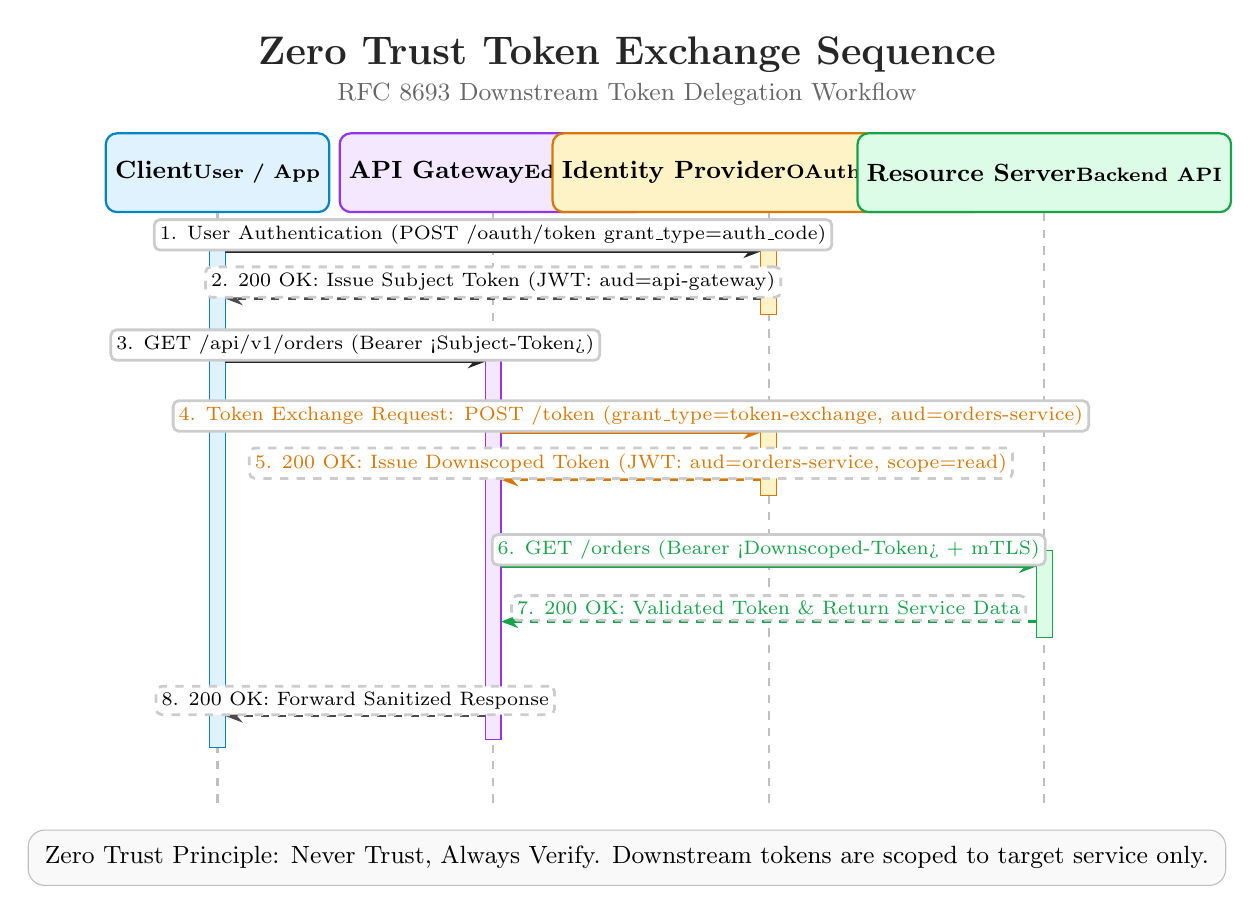
\begin{tikzpicture}[
  x=1cm, y=1cm, >=Stealth,
  lifeline/.style={draw=gray!50, dashed, line width=0.8pt},
  msg/.style={draw=black!85, line width=1pt, -{Stealth[length=2.2mm]}},
  reply/.style={draw=gray!60!black, dashed, line width=1pt, -{Stealth[length=2.2mm]}},
  lbl/.style={fill=white, draw=gray!40, rounded corners=2pt, font=\scriptsize, inner sep=2pt},
  partbox/.style 2 args={rectangle, draw=#1, fill=#2, thick, rounded corners=4pt, text centered, minimum width=2.5cm, minimum height=1.0cm, font=\bfseries\small}
]

  % Title
  \node[font=\bfseries\Large, text=black!85] at (5.2, 5.0) {Zero Trust Token Exchange Sequence};
  \node[font=\small, text=gray!80!black] at (5.2, 4.5) {RFC 8693 Downstream Token Delegation Workflow};

  % Participant Header Boxes
  \node[partbox={clientborder}{clientbg}] (client) at (0, 3.5) {Client\\ \scriptsize User / App};
  \node[partbox={gwborder}{gwbg}] (gw) at (3.5, 3.5) {API Gateway\\ \scriptsize Edge PEP};
  \node[partbox={idpborder}{idpbg}] (idp) at (7.0, 3.5) {Identity Provider\\ \scriptsize OAuth 2.0 / STS};
  \node[partbox={rsborder}{rsbg}] (rs) at (10.5, 3.5) {Resource Server\\ \scriptsize Backend API};

  % Lifelines
  \draw[lifeline] (client.south) -- (0, -4.5);
  \draw[lifeline] (gw.south) -- (3.5, -4.5);
  \draw[lifeline] (idp.south) -- (7.0, -4.5);
  \draw[lifeline] (rs.south) -- (10.5, -4.5);

  % Activation Bars
  \filldraw[fill=clientbg, draw=clientborder] (-0.1, 2.7) rectangle (0.1, -3.8);
  \filldraw[fill=gwbg, draw=gwborder] (3.4, 1.3) rectangle (3.6, -3.7);
  \filldraw[fill=idpbg, draw=idpborder] (6.9, 2.7) rectangle (7.1, 1.7);
  \filldraw[fill=idpbg, draw=idpborder] (6.9, 0.4) rectangle (7.1, -0.6);
  \filldraw[fill=rsbg, draw=rsborder] (10.4, -1.3) rectangle (10.6, -2.4);

  % ==================== SEQUENCE STEPS 1 TO 8 ====================

  % Step 1: Client -> IdP
  \draw[msg] (0.1, 2.5) -- (6.9, 2.5)
    node[midway, above, lbl] {1. User Authentication (POST /oauth/token grant\_type=auth\_code)};

  % Step 2: IdP -> Client
  \draw[reply] (6.9, 1.9) -- (0.1, 1.9)
    node[midway, above, lbl] {2. 200 OK: Issue Subject Token (JWT: aud=api-gateway)};

  % Step 3: Client -> API Gateway
  \draw[msg] (0.1, 1.1) -- (3.4, 1.1)
    node[midway, above, lbl] {3. GET /api/v1/orders (Bearer <Subject-Token>)};

  % Step 4: API Gateway -> IdP (Token Exchange)
  \draw[msg, color=idpborder] (3.6, 0.2) -- (6.9, 0.2)
    node[midway, above, lbl, text=idpborder] {4. Token Exchange Request: POST /token (grant\_type=token-exchange, aud=orders-service)};

  % Step 5: IdP -> API Gateway
  \draw[reply, color=idpborder] (6.9, -0.4) -- (3.6, -0.4)
    node[midway, above, lbl, text=idpborder] {5. 200 OK: Issue Downscoped Token (JWT: aud=orders-service, scope=read)};

  % Step 6: API Gateway -> Resource Server
  \draw[msg, color=rsborder] (3.6, -1.5) -- (10.4, -1.5)
    node[midway, above, lbl, text=rsborder] {6. GET /orders (Bearer <Downscoped-Token> + mTLS)};

  % Step 7: Resource Server -> API Gateway
  \draw[reply, color=rsborder] (10.4, -2.2) -- (3.6, -2.2)
    node[midway, above, lbl, text=rsborder] {7. 200 OK: Validated Token \& Return Service Data};

  % Step 8: API Gateway -> Client
  \draw[reply] (3.4, -3.4) -- (0.1, -3.4)
    node[midway, above, lbl] {8. 200 OK: Forward Sanitized Response};

  % Bottom Principle Note
  \node[draw=gray!50, fill=gray!5, rounded corners=6pt, font=\small, inner sep=6pt] at (5.2, -5.2) {
    Zero Trust Principle: Never Trust, Always Verify. Downstream tokens are scoped to target service only.
  };

\end{tikzpicture}
\end{document}
